% Compilé avec lualatex

\documentclass{beamer}

\usepackage[utf8]{inputenc}
\usetheme{Singapore}
\usepackage{xcolor}
\setbeamertemplate{footline}[frame number]

\usepackage{mathlist}

\usepackage[utf8]{inputenc}
\usepackage{amsmath,amssymb}

\newtheorem{defi}{Definition}
\newtheorem{theo}{Theorem}
\newtheorem{coro}{Corollaire}
\newtheorem{lem}{Lemme}

%\usepackage{doublespace}
\usepackage{epic,eepic}
\usepackage{pstricks, pst-tree}

\usepackage{times}

\usepackage{ulem}
\usepackage{crayola}

\usepackage{listings}
%\topmargin=-0.6in
\lstloadlanguages{C++}
\lstset{language=C++}
%%}

\setbeamercovered{dynamic}

\def\bxi{\boldsymbol\xi}
\def\bepsilon{\boldsymbol\epsilon}
\def\bomega{\boldsymbol\omega}

\def\cB{\mathcal{B}}

\def\aff{\operatorname{aff}}

\usepackage{tcolorbox}
\tcbuselibrary{theorems}

\newcommand{\tim}[1]{\;\; \mbox{#1} \;\;}

\def\cN{\mathcal{N}}

\title[Adaptive methods]{Stochastic programming\\SAA: adaptive sampling}

\author[Fabian Bastin]{Fabian Bastin \\ \url{bastin@iro.umontreal.ca} \\ Université de Montréal -- CIRRELT -- IVADO -- Fin-ML}

\date{}

\begin{document}

\frame{\titlepage}

\begin{frame}
\frametitle{Motivation}

\underline{Reminder}: we consider the stochastic problem
\[
\textcolor{red}{\min_{x \in S} g(x) = E_P \left[ G(x, \bxi) \right]},
\]
where
\begin{itemize}
	\item
	$x \in \rit^m$
	\item
	$S$ is a compact subset of $\rit^m$
	\item
	$\bxi$ is a real random vector defined on $( \Xi, \mathcal{F}, P )$ and taking values in $( \rit^k, \mathcal{B}^k )$ ($\mathcal{B}^k$ is the Borel measure)
	\item
	$G: \rit^m \times \rit^k \rightarrow \rit$
\end{itemize}

Sample average approximation:
\[
\min_{x \in S} \hat{g}_N(x) = \frac{1}{N} \sum_{i = 1}^N G (x, \xi_i),
\]

\end{frame}

\begin{frame}
\frametitle{Convergence}

In addition to our previous consistency results for $N \rightarrow \infty$, the central limit theorem tells us that, if the draws are independent and identically distributed (i.i.d.) (and finite $g(x)$),
\[
\sqrt{N} [ \hat{g}_N(x) - g(x) ] \Rightarrow N(0, \sigma^2(x)),
\]
where $\sigma^2(x) = \mbox{var}(G(x,\xi))$, and $\Rightarrow$ denotes convergence in distribution.

\mbox{}

This result is only valid for a given $x$.
It is necessary to set stronger conditions in order to have a functional convergence.

\mbox{}

Note: under our assumptions, $\hat{g}_N(x)$ is continuous over $S$, and can thus be considered as a point in the Banach space $C(s)$.

\end{frame}

\begin{frame}
\frametitle{Banach space $C(s)$}

$C(S)$ is the space of continuous functions $\psi: S \rightarrow \rit$,
equipped with the sup-norm $\| \psi \| := \sup_{x \in S}| \psi |$

\mbox{}

$C(S)$ is a Banach space, i.e. a normed vectorial space, complete under the distance issued from its norm.
A metric space $M$ is said complete or complete space if every Cauchy suite in $M$ has a limit in $M$ (i.e. it converges in $M$).

\mbox{}

We will extend the (pointwise) central limit theorem to a functional central limit theorem, assuming as usual that the draws are i.i.d.

\end{frame}

\begin{frame}
\frametitle{Assumptions}

\begin{enumerate}
\item
$\forall\, x \in S$, $G(x,\cdot)$ is measurable (i.e. its expectation exists).
\item
$\exists \overline{x} \in S$ such that $E_P[G(\overline{x}, \xi)^2] < \infty$.
\item
(Lipschitz continuity condition) 
$\exists$ $K(\xi) \geq 0$ such that $E[K(\xi)]$ is finite, and
$\forall\, x_1$, $x_2 \in S$ and a.e. $\xi$,
\[
| G(x_1, \xi) - G(x_2, \xi) )| \leq K(\xi) \| x_1 - x_2\|,
\]
We assume moreover that $E[K^2(\xi)] < \infty$.% is finite.
\end{enumerate}

\end{frame}

\begin{frame}
\frametitle{Functional central limit theorem}

Under these conditions,
\[
N^{1/2} [\hat{g}_n - g] \Rightarrow Y \in C(S).
\]

\mbox{}

%Under the i.i.d. condition, for any points
If $x_1,\ldots,x_k \in S$, %the random vector 
$
(Y(x_1),\ldots,Y(x_k)) \sim N(0, \Sigma),
$
where $\Sigma$ is the covariance matrix from $(G(x_1, \xi), \ldots, G(x_k, \xi))$.
% follows a multivariate normal distribution, with the covariance matrix corresponding to the covariance of the vector $(G(x_1, \xi), \ldots, G(x_k, \xi))$.

\mbox{}

If $N^{1/2}(\hat{g}_N - g) \Rightarrow Y \in C(S)$ (with $\lbrace \hat{g}_n \rbrace$ and $g$ in $C(S)$), and
\[
\hat{v}_N = \min_{x \in S} \hat{g}_N(x) \mbox{ et } v^*= \min_{x \in S} g(x),
\]
then
\[
N^{1/2}(\hat{v}_N - v^*) \Rightarrow \min_{x \in S^*} Y(x).
\]

\end{frame}

\begin{frame}
\frametitle{Convergence of global solutions}

If $S^*$ is a singleton, under the previous assumptions, in the i.i.d. case,
\[
N^{1/2}(\hat{v}_n - v^*) \Rightarrow N(0, \sigma^2(x^*) ).
\]

\mbox{}

Under some additional conditions, we also have the convergence of $E[\hat{v}_N]$ to $v^*$.

\mbox{}

But all these results become difficult to extend in the case of local optimization.

\mbox{}

However, we see that the results should be better with larger $N$, but at a higher computational cost, as
$$
\hat{g}_N(x) = \frac{1}{N} \sum_{i = 1}^N G (x, \xi_i).
$$

\end{frame}

\begin{frame}
\frametitle{External adaptive method}
%\frametitle{Convergence of global solutions (cont'd)}

What does interest us?
\[
\textcolor{red}{\min_{x \in S}}\ \hat{g}_N(x) = \frac{1}{N} \sum_{i = 1}^N G (x, \xi_i).
\]
%In other terms, for a given approximation level defined by the number of random draws, it is possible to speed up the first iterations of the optimization process by considering subsets of the sample.

\mbox{}

%Alternatively,
We can start with a small sample and extend if over the iterations:
the adaptive sampling procedure can be \textcolor{blue}{external} to the algorithm, or \textcolor{blue}{internal}.
%\\
%Therefore, there are \textcolor{red}{several possible strategies}.

\mbox{}

An external approach is known as \textcolor{red}{retrospective approximation} consists to repeatedly apply the optimization algorithm with samples of increasing sizes.

\end{frame}

\begin{frame}
\frametitle{Retrospective approximation (RA)}

Introduced by Healy and Schruben in 1991.

\mbox{}

Let $k$ be the iteration index. Components:
\begin{enumerate}
	\item 
	A procedure for solving a generated sample-path problem to specified tolerance vector $\epsilon_k$, delivering a solution $x_k$.
	\item
	A sequence $\{ N_k \}$ of sample sizes tending to infinity.
	\item
	A sequence $\{ \epsilon_k \}$ of error-tolerances tending to zero.
	\item
	A sequence of weights $\{ w_{kj},\ j = 1, 2,\ldots, k \}$ for each iteration.
\end{enumerate}

\mbox{}

We define
%$\overline{X}_k$ as the weighted sum of
%retrospective solutions $\{ X_i,\ i = 1,\ldots,k \}$:
$$
\overline{x}_k := \sum_{j = 1}^k w_{kj} x_j.
$$
\end{frame}

\begin{frame}
\frametitle{Retrospective approximation: principle}

\begin{description}
\item[Step 0.]
Set $k = 1$ and choose $\overline{x}_0 = x_0 \in S$.
\item[Step 1.]
Generate a sample-path problem with sample size $N_k$, with a ``warm start'', i.e. starting from $\overline{x}_{k-1}$ % as the initial guess,
to solve the generated problem with the error-tolerance $\epsilon_k$.
Denote the obtained retrospective solution by $x_k$.
\item[Step 2.]
Compute the solution $\overline{x}_k$.
%as the weighted sum of
%retrospective solutions $\{ X_i,\ i = 1,\ldots,k \}$:
%$$
%\overline{X}_k = \sum_{j = 1}^k w_{kj} X_j.
%$$
\item[Step 3.]
Set $k \leftarrow k + 1$ and go to Step 1.
\end{description}

\end{frame}

\begin{frame}
\frametitle{Retrospective approximation: assumptions}

\begin{itemize}
\item
The true function $g$ has a unique minimizer $x^* \in S$.
\item
$G(\cdot,\xi)$ is Lipschitz with Lipschitz constant $L(\xi)$ on $S$ a.s., and $E[L(\xi)] < \infty$.
\item
$G(\cdot,\xi)$ is continuously differentiable at any $x \in \cB(x^*, \epsilon)$, $\epsilon > 0$, a.s.
\item
$\exists x \in S$ such that $E[\|\nabla_x G(x,\xi)\|^2] < \infty$.
\item
The sample function $\hat{g}_N(x)$ has a unique minimum $x_N^*$ a.s.
\item
When $\hat{g}_N(x)$ attains a unique minimum $X_N^*$, $\hat{g}_N(x)$ is twice differentiable at $x_N^*$.
Furthermore, the $\nabla^2 \hat{g}_N (x_N^*)$ is positive definite with smallest eigenvalue uniformly bounded away from 0 a.s.
\item
The solution $x_k$ obtained from the $k^{th}$ iteration of RA satisfies $\| \nabla \hat{g}_{N_k}(x_k) \| \leq \epsilon_k$.
\end{itemize}

\end{frame}

\begin{frame}
\frametitle{Retrospective approximation: assumptions}

\begin{itemize}
\item
The numerical procedure used to solve the sample-path problems in RA exhibits $p^{th}$-order sublinear convergence or $p^{th}$-order linear convergence with respect to the observed derivatives.
\item
The sample sizes are increased linearly, i.e., $N_k = c N_{k - 1} > 1$ for all $k$.
\item
The error-tolerances are chosen so that
$\epsilon_k= O(1/\sqrt{N_k})$.
\end{itemize}

\end{frame}

\begin{frame}
\frametitle{Retrospective approximation: convergence rate}

Under the previous assumptions, %the sequence of solutions obtained using the RA procedure satisfies
$$
C_k \| x_k - x^* \|^2 = O_p(1),
$$
as $k \rightarrow \infty$, where $C_k$ is the total amount of computational work done until the $k^{th}$ iteration and is given by $C_k = \sum^k_{i = 1} Q_iN_i$.
Here $Q_i$ is the number of points visited by the numerical procedure during the $i$th iteration.

\mbox{}

We recover the convergence rate of stochastic approximation method.

\end{frame}

%\begin{frame}
%\frametitle{External adaptive algorithm}

%\begin{description}
%\item[Step 0.] Step $k = 0$, $N_{\max}$ and $N_0$, with $0 < N_0 \leq N_{\max}$. Define some feasible point $\tilde{z}$.
%\item[Step 1.] (Approximativemly) solve $\hat{g}_{N_k}$ with $\tilde{z}$ as starting point and let $z^*_{N_k}$ denotes the found solution.
%\item[Step 2.] If $N_k = N_{\max}$, stop. Otherwise, set $N_{k+1}$ such that  $N_k < N_{k+1} < N_{\max}$, and $\tilde{z} = z^*_{N_k}$.
%Increment $k$ and return to Step~1.
%\end{description}

%\end{frame}

\begin{frame}
\frametitle{Internal-external adaptive method}

The major issue with this procedure is how to quantify the word ``approximative'' in Step~1.
If no care is taken, the resulting algorithm can in fact be more time-consuming that the direct minimization of $\hat{g}_{N_{\max}}$.

\mbox{}

We can also replace the stopping test on $N_{\max}$ by a test of the criticality conditions of optimality.

\mbox{}

The \textcolor{blue}{internal approach} is a non-monotone strategy that depends on the underlying optimization methods.
Here, we consider the unconstrained case.

\mbox{}

More precisely, we generate a sample before the optimization process, with $N_{\max}$ i.i.d. random draws.
At iteration $k$, we will use a subset of this initial sample, using $N_k$ of the $N_{\max}$ random draws, typically the first ones.

\end{frame}

\begin{frame}
\frametitle{Accuracy estimation}

%For simplicity, we will use the first $N_k$ random draws.
This implies that $\hat{g}_N$ is a smooth function, well defined for each choice of $N$.

%\mbox{}

In order to determine a sample size, we can measure the approximation accuracy.
Let $\alpha_{\delta}$ be the quantile of a $\cN(0,1)$ associated to some significance level $\delta$, i.e. $P_{\bxi} [ -\alpha_{\delta} \leq Y \leq \alpha_{\delta} ] = \delta$, where $Y \sim \cN(0,1)$.

\mbox{}

We will use the central limit theorem
\[
g(x) - \hat{g}_N(x) \Rightarrow \cN \left( 0, \frac{\sigma^2(x)}{N} \right),
\]
where $\sigma^2(x)$ is the variance of $g$, taken at the point $x$, in order to build a confidence interval for $g(x)$ around $\hat{g}_N(x)$, as
\[
[\hat{g}_N(x) - \epsilon^{\delta}_N(x),\ \hat{g}_N(x) + \epsilon^{\delta}_N(x)],
\]

\end{frame}

\begin{frame}
\frametitle{Accuracy estimation (cont'd)}

$\epsilon^{\delta}_N(x)$ is given by
\[
\epsilon_{\delta}^N(x) = \alpha_{\delta} \frac{\sigma(x)}{\sqrt{N}}.
\]

\mbox{}

Typically, we will choose $\alpha_{0.9} \approx 1.64$ or $\alpha_{0.95} \approx 1.96$.

\mbox{}

In practice, we do not know $\sigma^2(x)$, but we can use its estimator
\[
\hat{\sigma}^2_N(x) = \frac{1}{N-1}\sum_{i = 1}^N ( G(x,\xi_i) -
\hat{g}_N(x))^2.
\]

\mbox{}

We will exploit this error estimation in the context of trust-region methods.


\end{frame}

\begin{frame}
\frametitle{Basic principles}

The basic idea is that if the model approximates the objective function well enough w.r.t. the accuracy of the objective function (which depends on the sample size), we presume that we could work with a less accurate approximation, and therefore reduce the sample size.

\mbox{}

On the other hand, if the adequation of the model with respect to the accuracy of the objective function is poor, we can increase the sample size in an attempt to correct this deficiency.

\mbox{}

We assume the assumptions developed for the consistency analysis hold.

\mbox{}

A formal algorithm description follows.

\end{frame}

\begin{frame}
\frametitle{Algorithm BTRDA (Bastin, Cirillo, Toint, 2006)}

(Basic) trust-region algorithm with dynamic accuracy.

\mbox{}

\begin{description}
\item[Step 0. Initialization.]

initial point: $x_0$, initial trust-region radius: $\Delta_0$.
Set $\eta_1$ and $\eta_2$ such that $0 < \eta_1 \leq
\eta_2 < 1$ (for instance, $\eta_1 = 0.01$ and $\eta_2 = 0.75$),
%Define a minimum number of draws
$N_{\min} = N^0_{\min}$ and %a sample size
$N_0$ satisfying $\| \nabla \hat{g}_{N_0} (x_0) \| \ne 0$ if $\epsilon_{\delta}^{N_0}(x_{k+1}) \ne
0$, except if $N_0 = N_{\max}$.
Compute $\hat{g}_{N_0}(x_0)$ and set $k = 0$, $t = 0$.
\item[Step 1. Stopping test.]
Stop if $\| \nabla \hat{g}_{N_{k}}(x_{k})\| = 0$ and either
$N_k = N_{\max}$, either $\epsilon_{\delta}^{N_k}(x_k) = 0$.
Otherwise, go to Step 2.
\item[Step 2. Model definition]
Define a model $m_k^{N_k}$ of $\hat{g}_{N_k}(x)$ in $\mathcal{B}_k$.
Compute a new adequate sample size $N^{+}$, and set $N^- = N_k$.
\end{description}

\end{frame}

\begin{frame}
\frametitle{Algorithm BTRDA (cont'd)}

\begin{description}
\item[Step 3. Step computation]
Compute a step $s_k$ that sufficiently reduces $m_k^{N_k}$ and s.t. $x_k + s_k \in \mathcal{B}_k$.
Set
\[ \Delta m_k^{N_k} = m_k^{N_k}(x_k) - m_k^{N_k}(x_k+s_k). \]
\item[Step 4. Comparaison of decreases]
Compute $\hat{g}_{N^+} (x_k + s_k)$ and %define
\[
\rho_k = \frac{\hat{g}_{N_k}(x_k) - \hat{g}_{N^+}(x_k+s_k)}
{\Delta m_k^{N_k}}.
\]
\item[Step 5. Sample size update]
If $\rho_k < \eta_1$ and $N_k \ne N^+$, modify $N^-$ or the candidate sample size $N^+$ in order to take account of variance differences.
Update $\rho_k$.
\end{description}

\end{frame}

\begin{frame}
\frametitle{Algorithm BTRDA (cont'd)}

\begin{description}
\item[Step 6. Candidate iterate acceptance]
If $\rho_k < \eta_1$, define $x_{k+1} = x_k$, $N_{k+1} = N^-$.
Otherwise, define $x_{k+1} = x_k + s_k$ and set $N_{k+1} = N^+$;
increment $t$.

\mbox{}

If $N_{k+1} \ne N^{\max}$, $\| \nabla \hat{g}_{N_{k+1}}(x_{k+1})\| = 0$, and
$\epsilon_{\delta}^{N_{k+1}}(x_{k+1}) \ne 0$, increase $N_{k+1}$ to some size less or equal to $N_{\max}$ such that $\| \nabla \hat{g}_{N_{k+1}}(x_{k+1})\| \ne 0$ if $N_{k+1} \ne N_{\max}$, and compute $\hat{g}_{N_{k+1}}(x_{k+1})$.

\mbox{}

If $N_k = N_{k+1}$ or if a sufficient decrease has been observed since the last evaluation of $\hat{g}_{N_{k+1}}$, set $N_{\min}^{k+1} = N_{\min}^k$.
Otherwise, set $N_{\min}^{k+1} > N^k_{\min}$.
\end{description}

\end{frame}

\begin{frame}
\frametitle{Algorithme: BTRDA (cont'd)}

\begin{description}
\item[Step 7. Trust region radius update]
\[
\Delta_{k+1} \in \begin{cases}
[\Delta_k, \infty) & \mbox{if } \rho_k \geq \eta_2, \\
[\gamma_2 \Delta_k, \Delta_k] & \mbox{if } \rho_k \in [\eta_1, \eta_2),\\
[\gamma_1 \Delta_k, \gamma_2 \Delta_k] & \mbox{if } \rho_k < \eta_1,
\end{cases}
\]
\end{description}

\mbox{}

In this algorithm the variable $t$ is used to count the number of successful iterations.

\mbox{}

Note: the algorithms BTR and BTRDA coincide if we fixe $N_k$ to $N_{\max}$ for all $k \geq 0$.

\end{frame}

\begin{frame}
\frametitle{Variable sample size strategy}										

\begin{itemize}
	\item 
Before the optimization, the user chooses a maximal sample size $N_{\max}$ (for instance the number of observations).
	\item 
A minimum sample size $N^0_{\min}$. % is defined in order to allow the estimation of the accuracy.
\item
Define $N_0 = \max\lbrace N^0_{\min}, 0.1N_{\max}\rbrace$ if $\| \nabla \hat{g}_{N_0}(x_0) \| \ne 0$ and $\epsilon_{\delta}^{N_0}(x_0) \ne 0$, $N_0 = N_{\max}$ otherwise.
\end{itemize}

\end{frame}

\begin{frame}
\frametitle{Choice of $N^+$ in (Step 3)}										

Sample size required to obtain an accuracy equal to $\Delta m_k$:
\[
N^s = \max \left\lbrace N^k_{\min},
\left\lceil
\frac{\alpha^2_{\delta}  \hat{\sigma}^2_N(x)}{(\Delta m_k^{N_k})^2}
\right\rceil \right\rbrace.
\]
Set
$$
\tau_1^k = \frac{\Delta m_k^{N_k}}{\epsilon_\delta^{N_k} (x_k)},\qquad
\tau_2^k = \frac{N_k}{\min \lbrace N_{\max}, N^s \rbrace}.
$$

Set $N^+ = \max\lbrace N', N^k_{\min}\rbrace$, where
$$
N' =
\begin{cases}
	\min \left\lbrace \lceil \chi_1 N_{\max} \rceil, \lceil N^s
	\rceil \right\rbrace & \text{if } \tau_1^k \geq 1, \\
	\min \left\lbrace \lceil \chi_1 N_{\max} \rceil, \lceil \tau_1^kN^s
	\rceil  \right\rbrace &  \text{if } \tau_1^k < 1 \text{ and }
	\tau_1^k \geq  \tau_2^k,\\
	\lceil \chi_1 N_{\max} \rceil & \text{if }  \nu_1 \leq \tau_1^k <
	1\text{ and }\tau_1^k < \tau_2^k,\\
	N_{\max} & \text{if } \tau_1^k < \nu_1\text{ and }\tau_1^k < \tau_2^k.
\end{cases}
$$

%Define constants $\nu_1$ and $\chi_1$ such that $\nu_1, \chi_1 \in (0,1)$.
%Use $\epsilon_{\delta}^{N_k}(x)$ to estimate the 

\end{frame}

\begin{frame}
\frametitle{Variable sample size strategy (cont'd)}

A possible value for $\chi_1$ is 0.5.

\begin{itemize}
	\item 
$\tau_1^k \geq 1$: $\Delta m_k \geq$ estimated accuracy.
%, and we reduce the sample size to $\min\{ N^s, \lceil \chi_1 N_{\max}
%\rceil \}$.
%The idea to use $\lceil \chi_1 N_{\max} \rceil$ comes from the practical observation that imposing such a decrease in the suggested sample sizes delivers a better numerical performance.
\item
$\tau_1^k < 1$: $\Delta m_k <$ accuracy.
However, %since the sample has been generated before the optimization process,
a sufficient improvement during several consecutive iterations can lead to a significant decrease.% in comparison to the approximation accuracy, while keeping the computational cost lower than if $N_{\max}$ draws were used.
\begin{itemize}
\item 
If $\tau_1^k \geq \tau_2^k$, the ratio between the current sample size and the potential next one is smaller than the ratio between $\Delta m_k$ and the estimated error.
%If the sample size increases, the error decreases for a similar $\Delta m_j^{N_j}$ ($j \geq k$), and therefore $\tau_1^k$ increases.
We capitalize on $\tau_1^k$ by computing a sample size smaller than  $N^s$, such that an improvement of the order $\epsilon_\delta^{N_k}(z_k)$ would be reached in approximatively $\lceil \tau_1^k \rceil$ iterations if $\tau_1^j$ is similar to $\tau_1^k$ for $j$ close to $k$.
\item
If $\tau_1^k < \tau_2^k$, it can nevertheless be cheaper to continue to work with a smaller sample size, defined again as $\lceil \chi_1 N_{\max} \rceil$, as long as $\tau_1^k$ is greater to some threshold $\nu_1$ (for instance 0.2).
%Below this threshold, we consider that the decrease is too small compared to the accuracy, and we possiblty increase the sample size.
\end{itemize}
\end{itemize}

\end{frame}

\begin{frame}
\frametitle{Accuracy differences}

If $N^+$ is not equal to $N_k$, the computation of
\[
 \hat{g}_{N_k} (x_k) - \hat{g}_{N^+} ( x_k + s_k )
\]
is affected by the change in approximation variance.
This can lead to $\rho_k < \eta_1$, even if the model $m_k^{N_k}$ gives a good predicition for the sample size $N^k$.

%\mbox{}

%In particular, $\hat{g}_{N^+}(x)$ can be greater than $\hat{g}_{N_k}(x_k)$ for all $x$ in a neighborhood of $x_k$.
%It is therefore important to avoid such cases, motivating the new definition of $\rho_k$, as described hereafter.

\mbox{}

If $N^+ > N_k$, compute $\hat{g}_{N^+}(x_k)$, $\Delta m_k^{N^+}$ and
$\epsilon_{\delta}^{N^+}(x_k)$, otherwise if $N^+ < N_k$ compute $\hat{g}_{N_k}(x_k + s_k)$.
Set $N^-$ to $\max\lbrace N_k, N^+ \rbrace$, and %redefine
\[
\rho_k = \frac{\hat{g}_{N^-}(x_k+s_k) - \hat{g}_{N^-}(x_k)}{\Delta
m_k^{N^-}}.
\]

\end{frame}

\begin{frame}
\frametitle{Additional tricks}

\begin{itemize}
\item Minimum sample size update

We want to be sure to use a sample size equal to $N_{\max}$ during the final iteration, in order to work with the desired accuracy.
We increase $N_{\min}$ when the adaptive strategy does not deliver sufficient numerical gains, or simply by 1 at each iteration.

\item
Additional safeguards to avoid theoretical pathological cases (a critical point of the SAA with $N_k < N_{\max}$ is found).
\end{itemize}

\end{frame}

\begin{frame}
\frametitle{Convergence}

\begin{theo}
Under some regularity assumptions, if
\[
\exists \kappa > 0\text{ such that }
\epsilon_{\delta}^{N_k}(x_k) \geq \kappa,
\]
for all $k$ large enough, then, almost surely, the algorithm converges in a finite number of iterations with a final sample size equal to $N_{\max}$, or the number of iterations is infinite and there exists some $j$ such that for all the iterations $i$, $i \geq j$, $N_i$ is equal to $N_{\max}$.
\end{theo}
%Proof: see Bastin, Cirillo et Toint, {\sl An adaptive {Monte Carlo}
%  algorithm for computing mixed logit estimators}, Computational
%Management Science 3(1), pp. 55--79, 2006.

\end{frame}

\begin{frame}{Application to discrete choice theory}
		
			Discrete {\blue set of alternatives} available for individual $i$:
			$\mathcal{A}(i)$.
			
			\textcolor{orange}Example: Which mode of transport have you chosen to come?
			
			\vspace*{0.3cm}
			
			\begin{minipage}[c]{0.3\linewidth}
				\begin{center}
					\scalebox{0.8}{
						\psset{nodesep=0.5cm, treesep=0.4cm}
						\pstree[treemode=R, nodesep=3pt]{\Tr{\bf{i}}}{
							\TC~[tnpos=r]{\quad\bf{car}}
							\TC~[tnpos=r]{\quad\bf{train}}
							\TC~[tnpos=r]{\quad\bf{bus}}
							\TC~[tnpos=r]{\quad\bf{bike}}
							\TC~[tnpos=r]{\quad\bf{walk}}
						}
					}%
				\end{center}%
			\end{minipage}
			\begin{minipage}{0.68\linewidth}
				
				Each alternative has some utility.\\
				{\red Utility $U_{ij}$} of $A_j \in \mathcal{A}(i)$:
				$U_{i j} = V(\beta) + \boldsymbol{\epsilon}_{ij}.$\\
				$\beta$: parameters to be estimated.
				
				{\red rational individuals}: a person chooses
				the alternative of {\blue maximum utility}\\
				{\red $\rightarrow$} choice of $A_j$ if $U_{ij} \geq U_{in}, \forall A_n \in
				\mathcal{A}(i)$.
				
			\end{minipage}
			
				Important case: Gumbel distributed residuals $\epsilon_{ij}$ (mean 0,
				scale factor $\mu$):
				{\red $\rightarrow$ multinomial logit} (MNL).
				
				{\blue Probability} that individual $i$ choose $A_j$:
					\psframebox[fillstyle=solid, fillcolor=lightgray]{
					$P_{ij} = \frac{e^{\mu V_{ij}(\beta)}}{\sum_{n= 1}^N e^{\mu
							V_{in}(\beta)}}$
					}
		
\end{frame}

%%%%%%%%%%%%%%%%%%%%%%%%%%%%%%%%%%%%%%%%%%%%%%%%%%%%%%%%%%%%%%%%%%%%%%%%%%%%%%%%%%%%%%%%%%%%%%%

	\begin{frame}{Mixed Logit models}
		
		\begin{footnotesize}
			Allow {\red heterogeneity} in parameters inside the population.
			\begin{center}
				$\boldsymbol{\beta} = \beta(\boldsymbol{\gamma}, \theta)$,
			\end{center}
			$\boldsymbol{\gamma}$: {\blue random vector}, e.g. vector of independant
			$N(0,1)$);\\
			$\theta$: {\blue vector of parameters}, e.g. vector of means and std dev.
			
				Probability choice of $A_j$ by individual $i$:
				\begin{center}
					\psframebox[fillstyle=solid, fillcolor=lightgray]{
						$P_{ij} (\theta) = E_{\bxi} \left[ L_{ij} (\gamma, \theta)\ \right] =
						\int { L_{ij} (\gamma, \theta)} f(\gamma) d\gamma$
					}
				\end{center}
				
				This integral is approximated by
				\begin{center}
					\psframebox[fillstyle=solid, fillcolor=lightgray]{
						$SP_{ij_i}^{R} = \frac{1}{R} \sum_{r= 1}^R L_{ij_i} (\gamma_r, \theta)$
					}
				\end{center}

				{\red SAA} problem:
				\begin{center}
					\psshadowbox[fillstyle=solid, fillcolor=orange]{
						$\max_{\theta} \hat{g}_R(\theta) = \max_{\theta} SLL(\theta) =
						\max_{\theta} \frac{1}{N} \sum_{n = 1}^{N} \ln SP_{ij_i}^{R}$
					}
				\end{center}
			
				$\rightarrow$ suggests to consider {\blue stochastic programming}
				techniques.
			
		\end{footnotesize}
		
\end{frame}

\begin{frame}{Properties of Mixed Logit}
		
		\begin{footnotesize}
			{\blue Stochastic programming}:
			\begin{center}
				\psframebox[fillstyle=solid, fillcolor=lightgray]{
					$\min_z g(z) = \min_z E_{\bxi} \left[G(z,\boldsymbol{\xi})\right]$
				}
			\end{center}
			
			{\blue Mixed logit}:
			\begin{center}
				\psframebox[fillstyle=solid, fillcolor=lightgray]{
					$\max_{\theta} g\left(\theta\right) = \max_{\theta} LL(\theta) \notag
					= \frac{1}{n} \sum_n \ln E_{\bxi} \left[ L_{in} \left(
					\boldsymbol{\gamma}, \theta \right) \right]$
				}
			\end{center}
			
			\vspace*{0.5cm}
				Consistency properties can be adapted. Assume {\red $I$ fixed} and {\red
					$R$ grows toward $\infty$}.
				
				\begin{center}
					\psshadowbox[fillstyle=solid, fillcolor=gray]{
						\begin{minipage}[fillstyle=solid, fillcolor=orange]{0.9\textwidth}
							If $\theta^*_R$, $R=1,\ldots$, are first (second)-order critical for
							the corresponding SAA problem, under some regularity conditions, for
							almost every sequence of random draws, there exists some limit point
							$\theta^*$ of $\left( \theta_R^* \right)_{R=1}^{\infty}$ that is first
							(second)-order critical.
						\end{minipage}
					}
				\end{center}
			
		\end{footnotesize}
		
\end{frame}

%%%%%%%%%%%%%%%%%%%
% Error estimation
%%%%%%%%%%%%%%%%%%%

\begin{frame}{Error estimation}
		
		%\vspace*{-0.5cm}
		
		\begin{footnotesize}
			
			With an i.i.d. sample for each individual, we have, from the delta
			method (see for instance Shapiro and Rubinstein):
			\begin{center}
				\psframebox[fillstyle=solid, fillcolor=lightgray]{
					$LL(\theta) - SLL^R(\theta) \Rightarrow N \left(0, \frac{1}{I}
					\sqrt{ \sum_{i = 1}^I \frac{ \sigma^2_{ij_i} (\theta)}
						{R \left( P_{ij_i} (\theta) \right)^2 }} \right)$
				}
			\end{center}
			
			Asymptotic value of the confidence interval radius:
			\begin{center}
				\psframebox[fillstyle=solid, fillcolor=orange]{
					$\epsilon_{\delta} = \alpha_{\delta} \frac{1}{I} \sqrt{ \sum_{i=1}^I
						\frac{ \sigma^2_{ij_i}\left(\theta \right) }
						{R \left( P_{ij_i} (\theta) \right)^2} }$
				}
			\end{center}
			$\delta$: signification level; $\alpha_{0.9} \approx 1.65$.
			
				Bias of simulation (Taylor expansion):
				\begin{center}
					\psframebox[fillstyle=solid, fillcolor=orange]{
						$B := E[SLL^R(\theta)] - LL(\theta) =
						-\frac{I\epsilon_{\delta}^2}{2\alpha_{\delta}^2}$
					}
				\end{center}
				
				In practice, use of SAA estimators $\sigma^R_{ij_i}(\theta)$ and $P^R_{ij_i}(\theta)$.
			
		\end{footnotesize}
		
\end{frame}

\begin{frame}{Algorithms comparison}
		
		\begin{footnotesize}
			
			5000 individuals, 5 alternatives, coefficients~$\sim N(0.5,1)$
			
			\begin{center}
				\hspace*{\stretch{1}}
				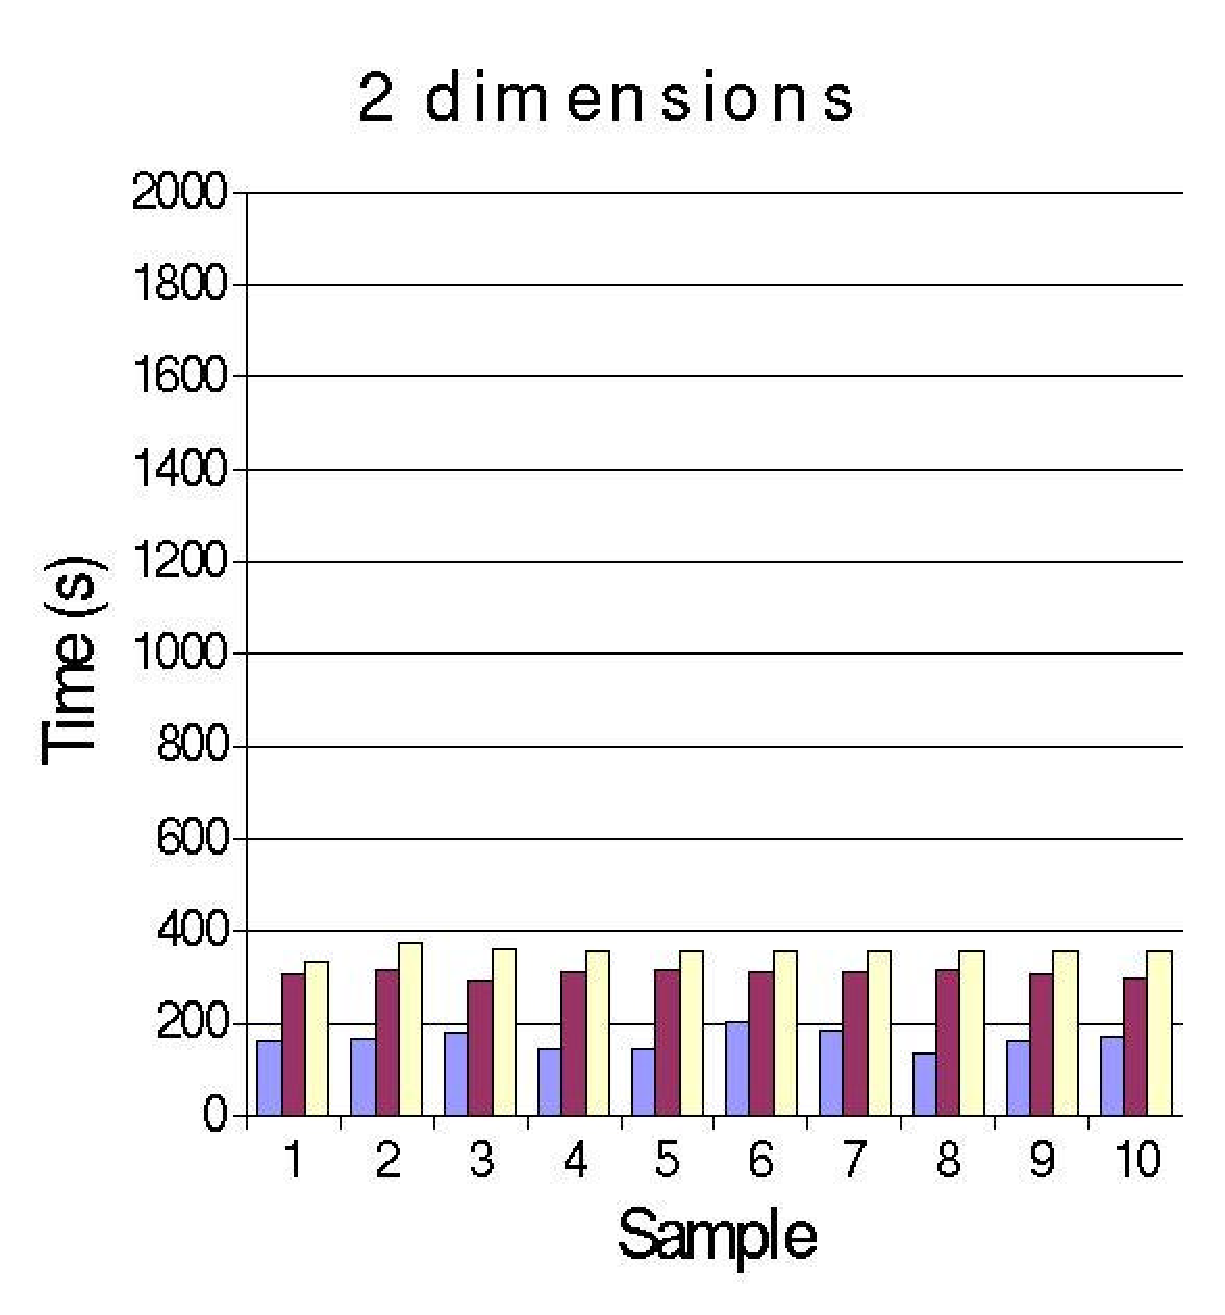
\includegraphics[width=0.30\linewidth]{2dims.eps}
				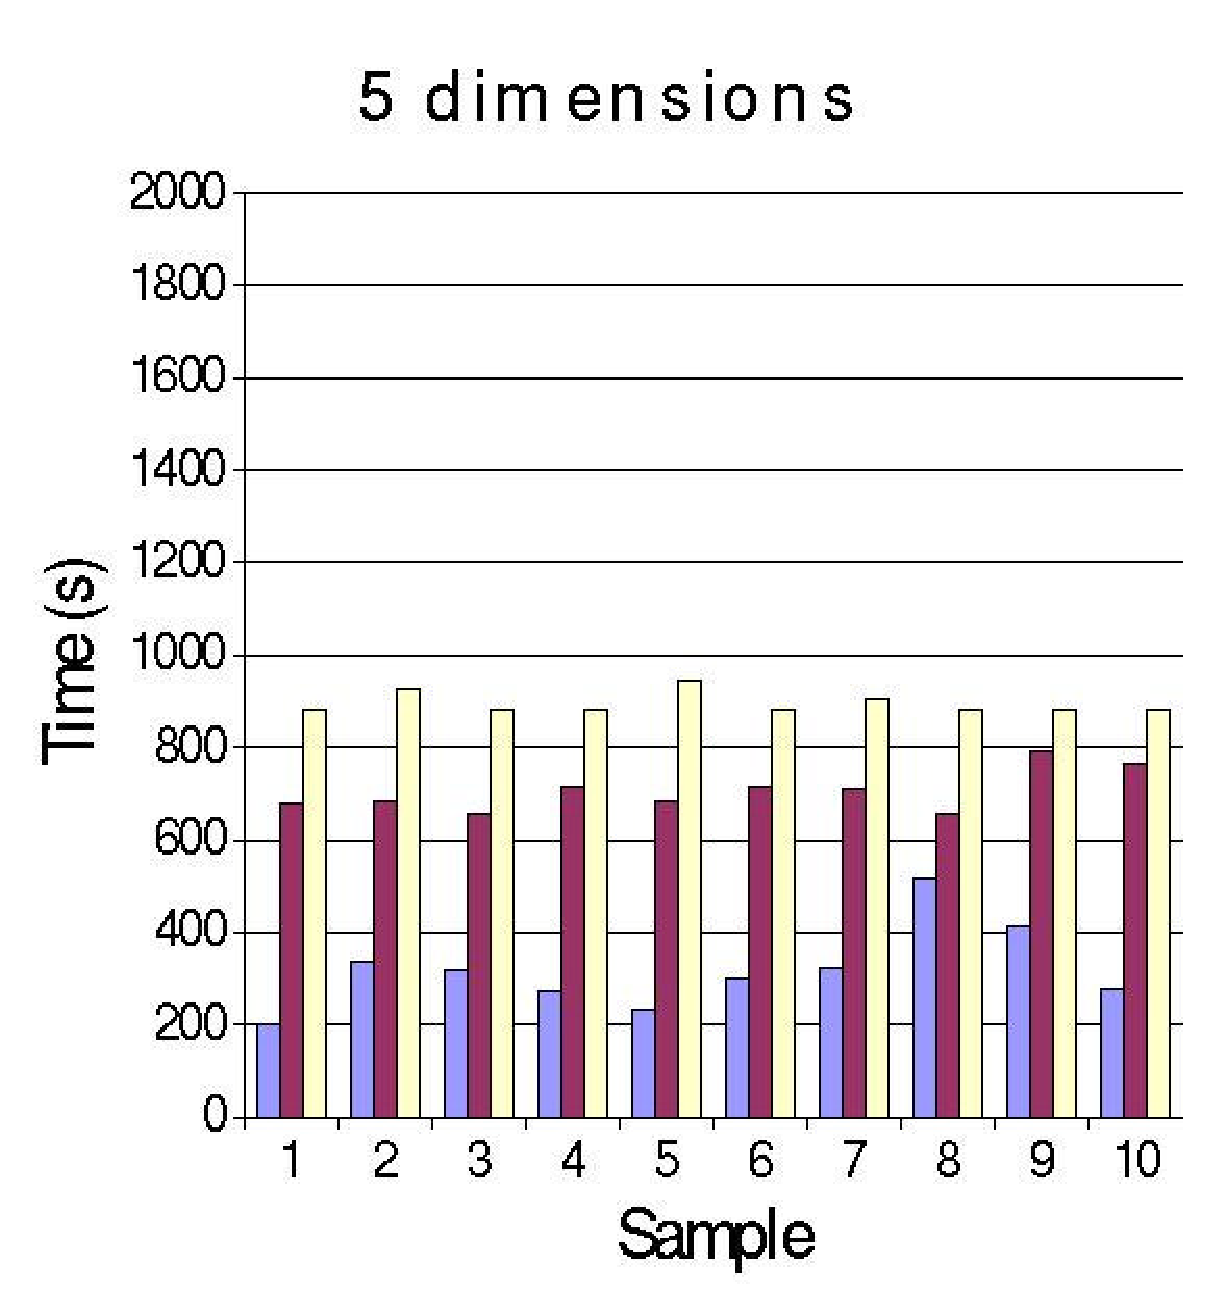
\includegraphics[width=0.30\linewidth]{5dims.eps}
				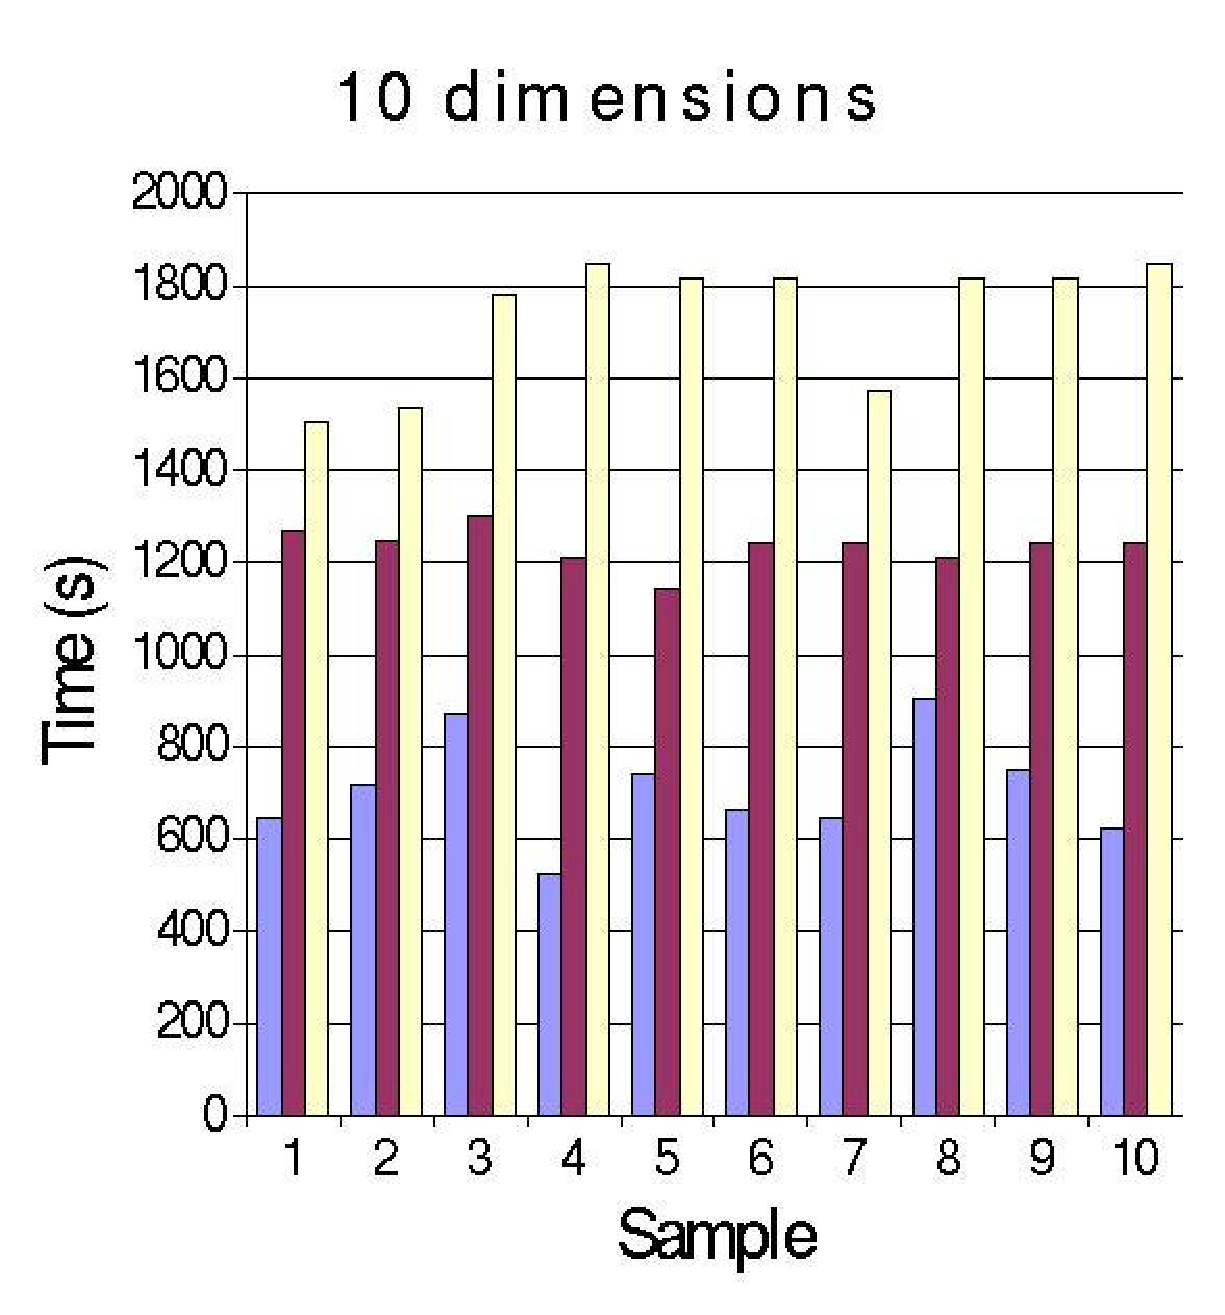
\includegraphics[width=0.30\linewidth]{10dims.eps}
				\hspace*{\stretch{1}}
				
				\vspace*{-0.2cm}
				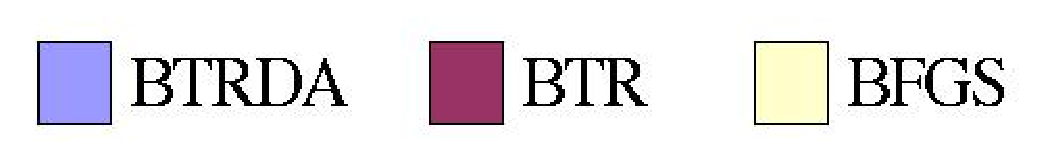
\includegraphics[width=0.3\linewidth]{legend.eps}
			\end{center}
			
				\begin{center}
					\vspace*{0.2cm}
%					\begin{spacing}{0.8}
						\begin{tabular}{|c|c|c|c|}
							\cline{2-4}
							\multicolumn{1}{c|}{} & 2 dimensions & 5 dimensions & 10 dimensions \\
							\hline
							\texttt{BTRDA} & $167s$ & $319s$ & $709s$ \\
							\texttt{BTR}   & $310s$ & $706s$ & $1235s$ \\
							\texttt{BFGS}  & $357s$ & $894s$ & $1736s$ \\
							\hline
						\end{tabular}
%					\end{spacing}
					
					\vspace*{0.4cm}
					
				\end{center}
				
				Results obtained with a Pentium IV, 2 Ghz. BFGS method has been implemented
				using the More-Thuente linesearch.
			
		\end{footnotesize}
		
\end{frame}


\begin{frame}[fragile]
\frametitle{Example}

%Mode choice model: \textcolor{blue}{Mobidrive} data (Axhausen et al., 2002)\\
%$N = 5799$ observations, $R_{\max} = 2000$ draws per individual, 14 parameters (integration dimension: 3 normal variables).
Mode choice model: {\blue Mobidrive} data (Axhausen
and al.)\\
{\red $\rightarrow$} 5799 observations;\\
{\red $\rightarrow$} 5 alternatives;\\
{\red $\rightarrow$} 14 parameters (3 random, normally distributed).

\begin{center}
\begin{minipage}{0.49\linewidth}
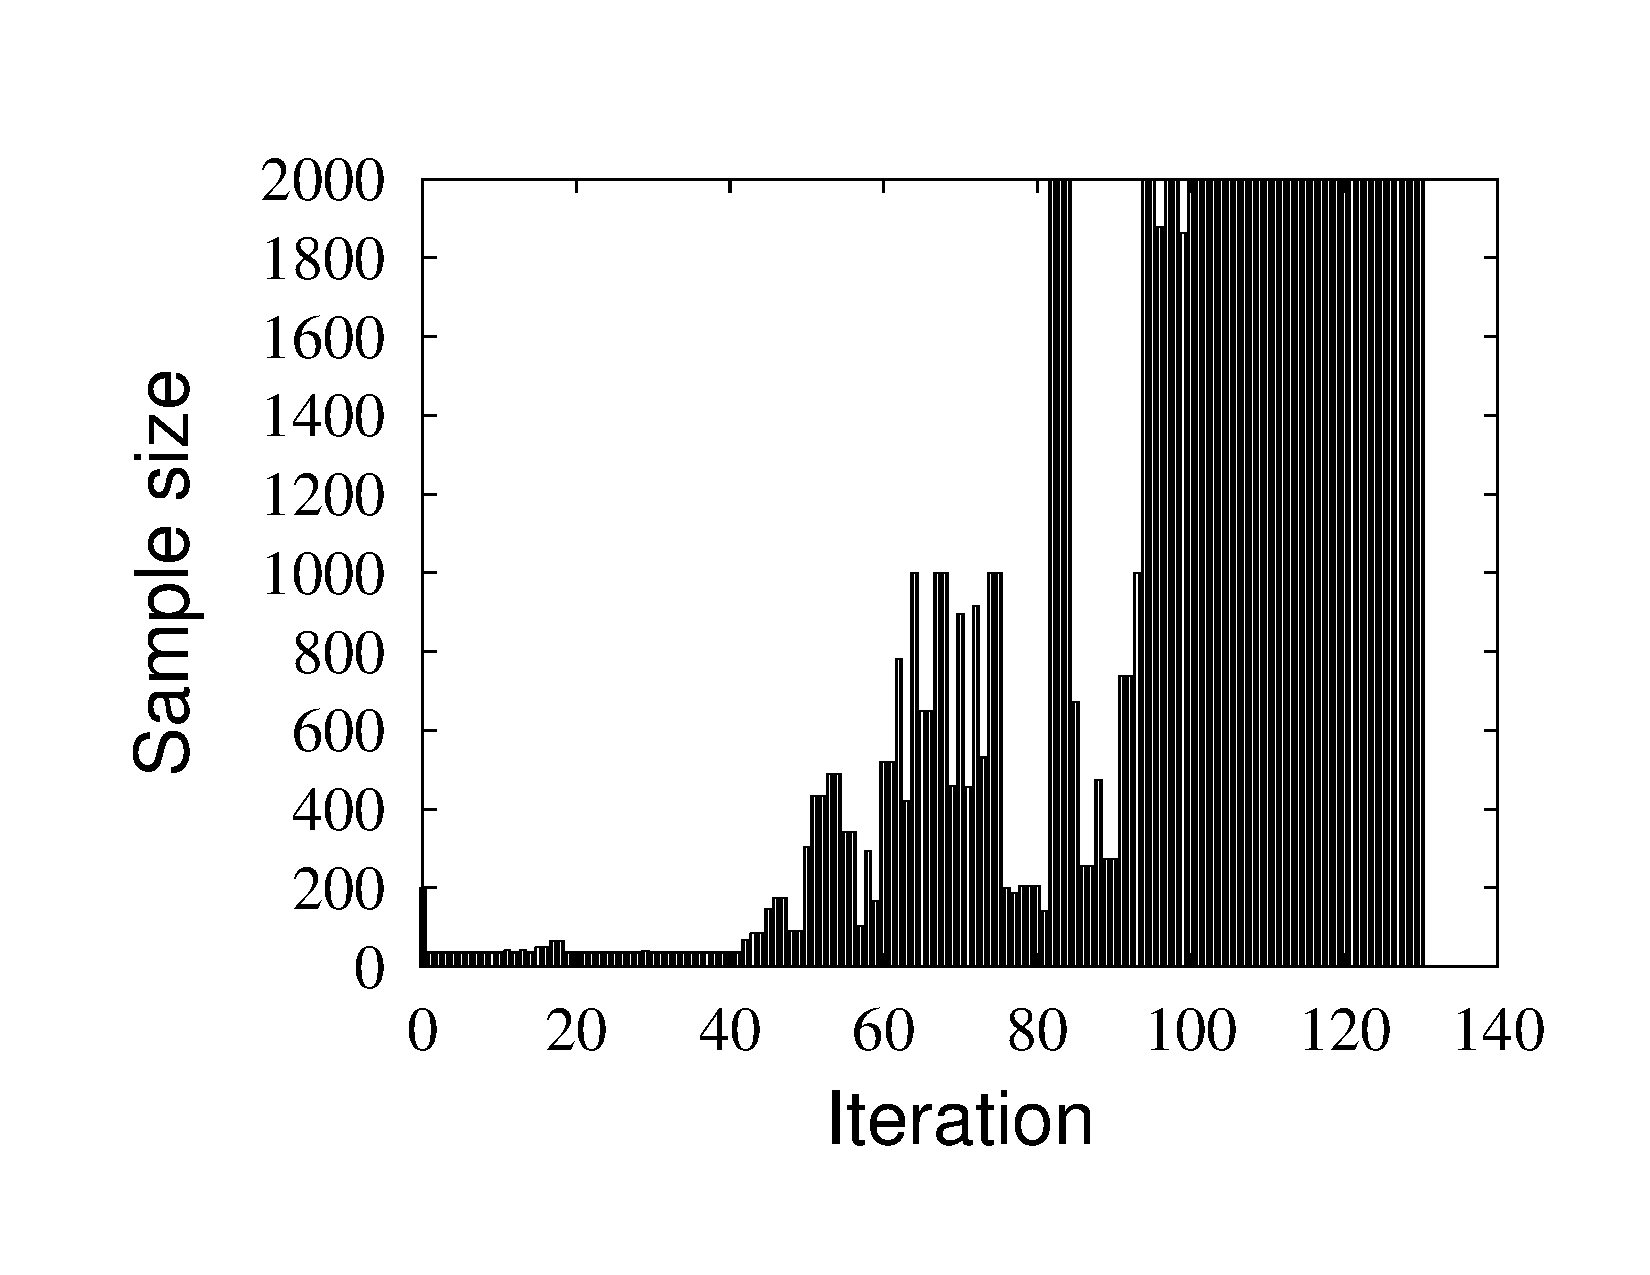
\includegraphics[width=\linewidth]{2000_sample_iter.pdf}
\end{minipage}
\begin{minipage}{0.49\linewidth}
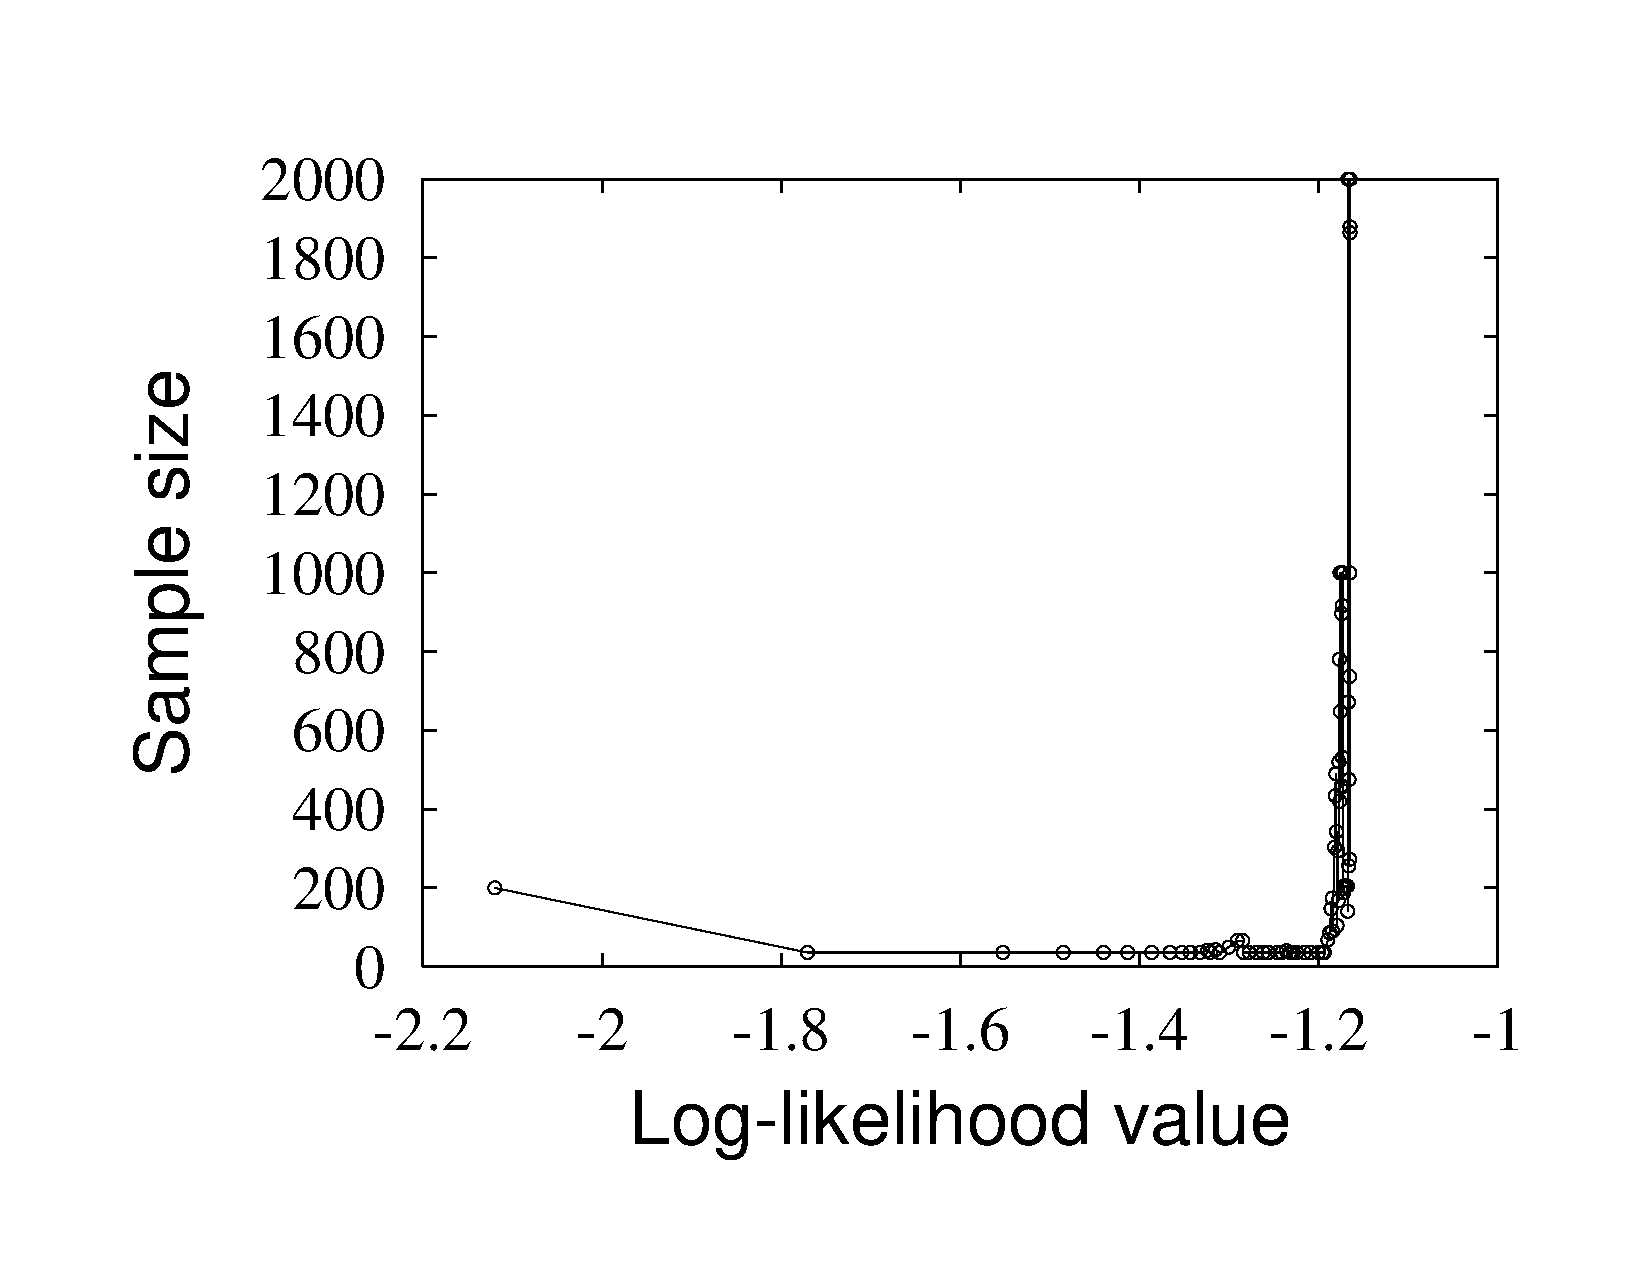
\includegraphics[width=\linewidth]{2000_sample_fct.pdf}
\end{minipage}
\end{center}
\begin{tiny}
{%\red
\hspace*{6.8cm}$\downarrow$\hspace*{3cm}$\downarrow$\\
\hspace*{6.0cm}Starting value\hspace*{1.2cm}Maximum value\\
}
\end{tiny}

\end{frame}

\begin{frame}{Possible improvement: how to draw samples?}
	
	\textcolor{red}{Sampling methods are notorious for generalization issues.}
	Common strategies:
	\begin{itemize}
		\item \textit{Independent Random Numbers} (IRN) (e.g. stochastic gradient descent)
		\item Incremental \textit{Common Random Numbers} (CRN): take the first $N_K$ numbers from a predefined sequance of random draws: $\mathcal{N}_k = \{ \xi_1, \ldots, \xi_{N_k} \}$
	\end{itemize}
	
\end{frame}

\begin{frame}{Incremental Common Random Numbers}    
	\centering
	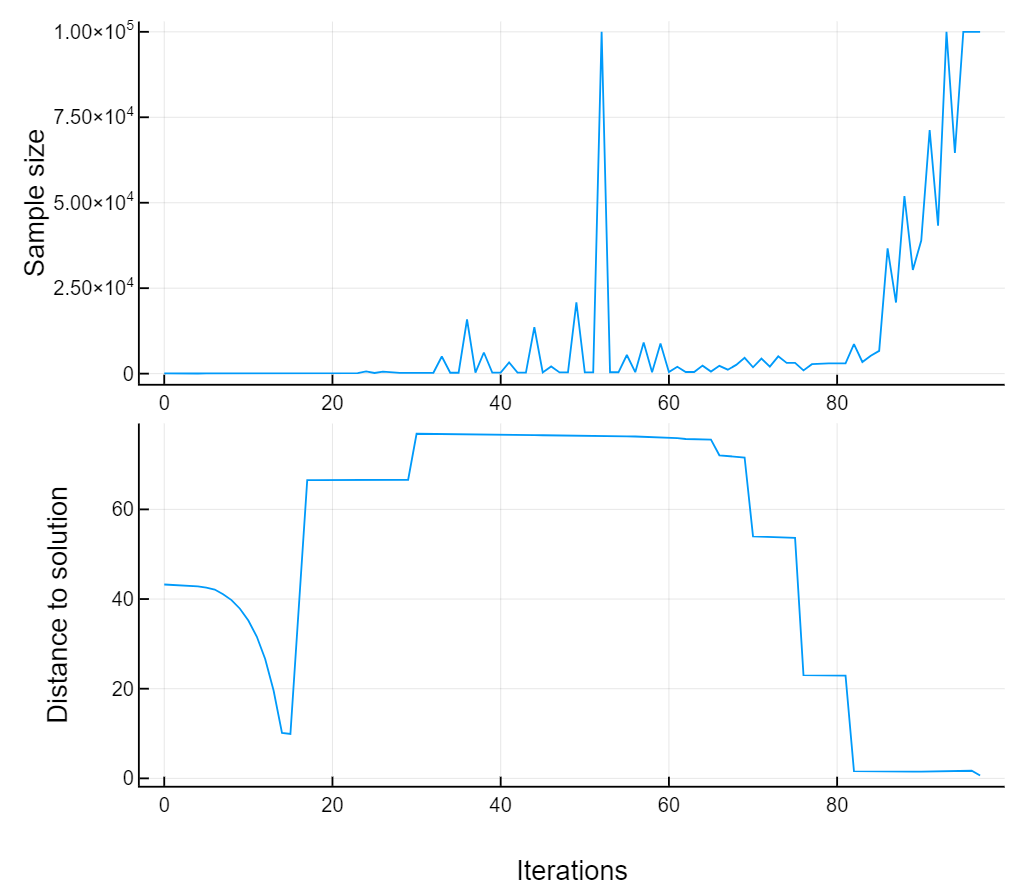
\includegraphics[scale=0.5]{DistTo_sampleSize_CRN.PNG}
\end{frame}

\begin{frame}{IRN/CRN combination (I/CRN)}
	
	\begin{enumerate}
		\item $N_{k+1} > N_k$
		
		Draw new samples $\xi_{N_{k}+1,\ldots,N_{k+1}}$ and set
		$$
		\mathcal{N}_{k+1} = \mathcal{N}_k \bigcup \left\{ \xi_{N_{k}+1,\ldots,\xi_{N_{k+1}}} \right\}.
		$$
		
		\item $N_{k+1} < N_k$
		$$\mathcal{N}_{k+1} = \mathcal{N}_k \backslash  \{\text{unformly randomly selected elements in } \mathcal{N}_k\}$$
	\end{enumerate}
	
	This heuristic reduces the risk to be trapped in a local minimizer or a saddle point.
	
\end{frame}

\end{document}